\documentclass[10pt,a4paper,twocolumn]{fullarticle}

\geometry{top=1.5cm,bottom=1.5cm,left=1.5cm,right=1.5cm}

\usepackage[british]{babel}
\usepackage{csquotes}

\usepackage{debug}
\usepackage{sciencestuff}

%---- SETUP

\title{Machine Learning for Level Truncation in Open String Field Theory \\[0.5em]
       {\Huge \bf Notes}}
\author{Harold Erbin}
\author{Riccardo Finotello}
\affil{%
  Dipartimento di Fisica, Universit\`{a} di Torino\authorcr{}
  and I.N.F.N. - sezione di Torino\authorcr{}
  Via P. Giuria 1, I-10125 Torino, Italy
}

\addbibresource{report.bib}

\begin{document}

  \pagestyle{plain}

  \twocolumn[
    \vspace*{-3em}
    \maketitle
  ]

  \section{Synopsis}\label{sec:syn}
    In the framework of bosonic Open String Field Theory (OSFT) we consider the
solutions at different radii of several observables and at different mass level
truncations.
We then use machine learning (ML) techniques to extract the value of the
observable at infinite mass level truncation.
More details can be found looking at the analysis at
\href{https://thesfinox.github.io/ml-sft-trunc/}{this URL} (only the analysis
is accessible, while the original database is not public).


  \section{Preliminary Operations}\label{sec:prel}
    \subsection{Description}\label{sec:prel:desc}

The dataset is composed of 46 different solutions at different radii. Each of
them is then composed of lists of several observables of different lengths
(varying from 15 to 21 entries each, as shown in \Cref{fig:prelim:length}).
\begin{figure}[htbp]
  \centering
  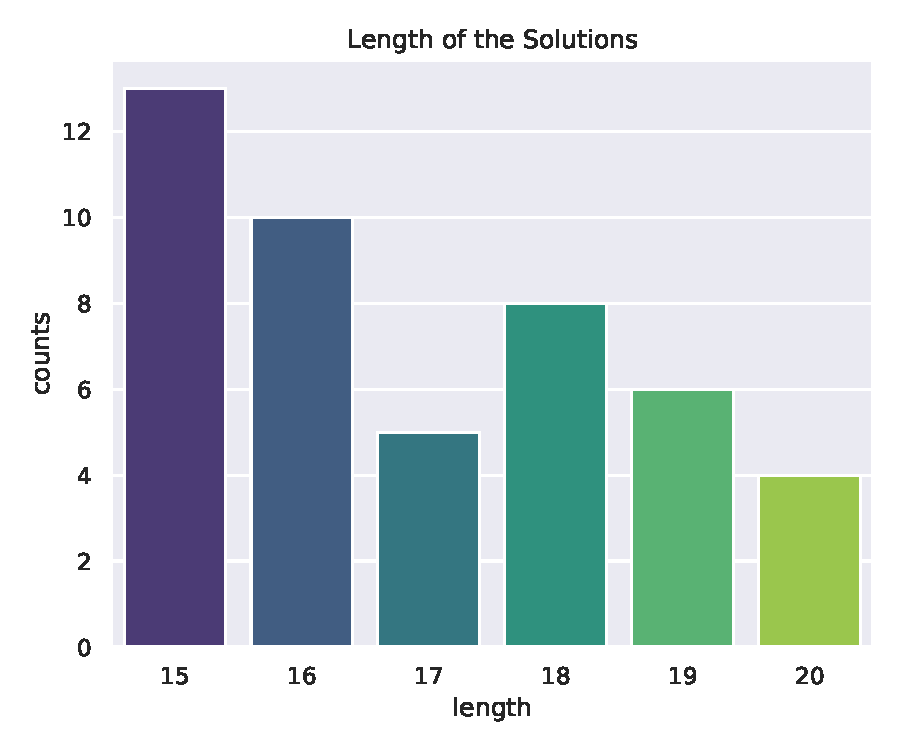
\includegraphics[width=0.4\textwidth]{img/length-solutions}
  \caption{Length of the solutions in the untidied dataset.}
  \label{fig:prelim:length}
\end{figure}
Every observable is characterised by its conformal weight (the \texttt{weight}
column in the dataset), its kind of ``oscillations'' (\texttt{type} variable,
categorical and ordered), its initialisation point (\texttt{init}) and the
truncation levels (from level 2 to level 18).
The objective of the analysis is the prediction of the extrapolation for the
level-$\infty$ truncation hosted in the \texttt{exp} variable of the dataset and which take 3 possible integer values in the range $[-1, 1]$.

\subsection{Input Preparation}\label{sec:prel:prep}

For the analysis we extract each entry of the lists and put it in separate
entry of the dataset: we first artificially insert a new variable labelling the
solution with a number from 0 to 45 and then flatten the dataset over the rows.
This way all columns hold only numerical variables which can be used for
different steps of the analysis.
The tidy dataset is composed of 778 samples over 22 columns (including the
newly created \texttt{solutions} variable).

We then look for duplicates inside the tidy dataset: rows which present exactly
the entries over all the columns, and exclude them from the analysis (we keep
only the first occurrence).
The final version of the dataset holds 732 samples and can be used for the
exploratory data analysis (EDA).


  \section{Exploratory Data Analysis}\label{sec:eda}
    During the EDA we study properties of the entries of the tidy dataset.
In particular we focus on outlier detection, distribution of the features,
correlations between variables, principal components and clustering.
We also anticipate that we will not use the \texttt{solutions} and
\texttt{init} variables in the regression analysis and as such we do not
include them in the EDA as well: they only serve as labels for the
identification of the entries.

\subsection{Outliers Detection}\label{sec:eda:outliers}

We perform outliers detection using the definition of the
\textit{interquartile} range, typical in statistical analysis.
This is defined as the interval between the 25th and 75th percentile of the
sample distribution, and outlying samples are entries greater or lower than 1.5
times such interval with respect to the sample mean.

We apply this procedure for each column in the dataset and compute the average
quantity of outlying samples for each variable: the truncation levels hold
between 17\% and 27\% of outliers in their distributions, while \texttt{weight}
holds only 6\% of outliers with respect to its distribution (the \texttt{type}
feature is categorical and as such there is no point in studying the outlying
samples for it). 
\begin{figure}[htbp]
  \centering
  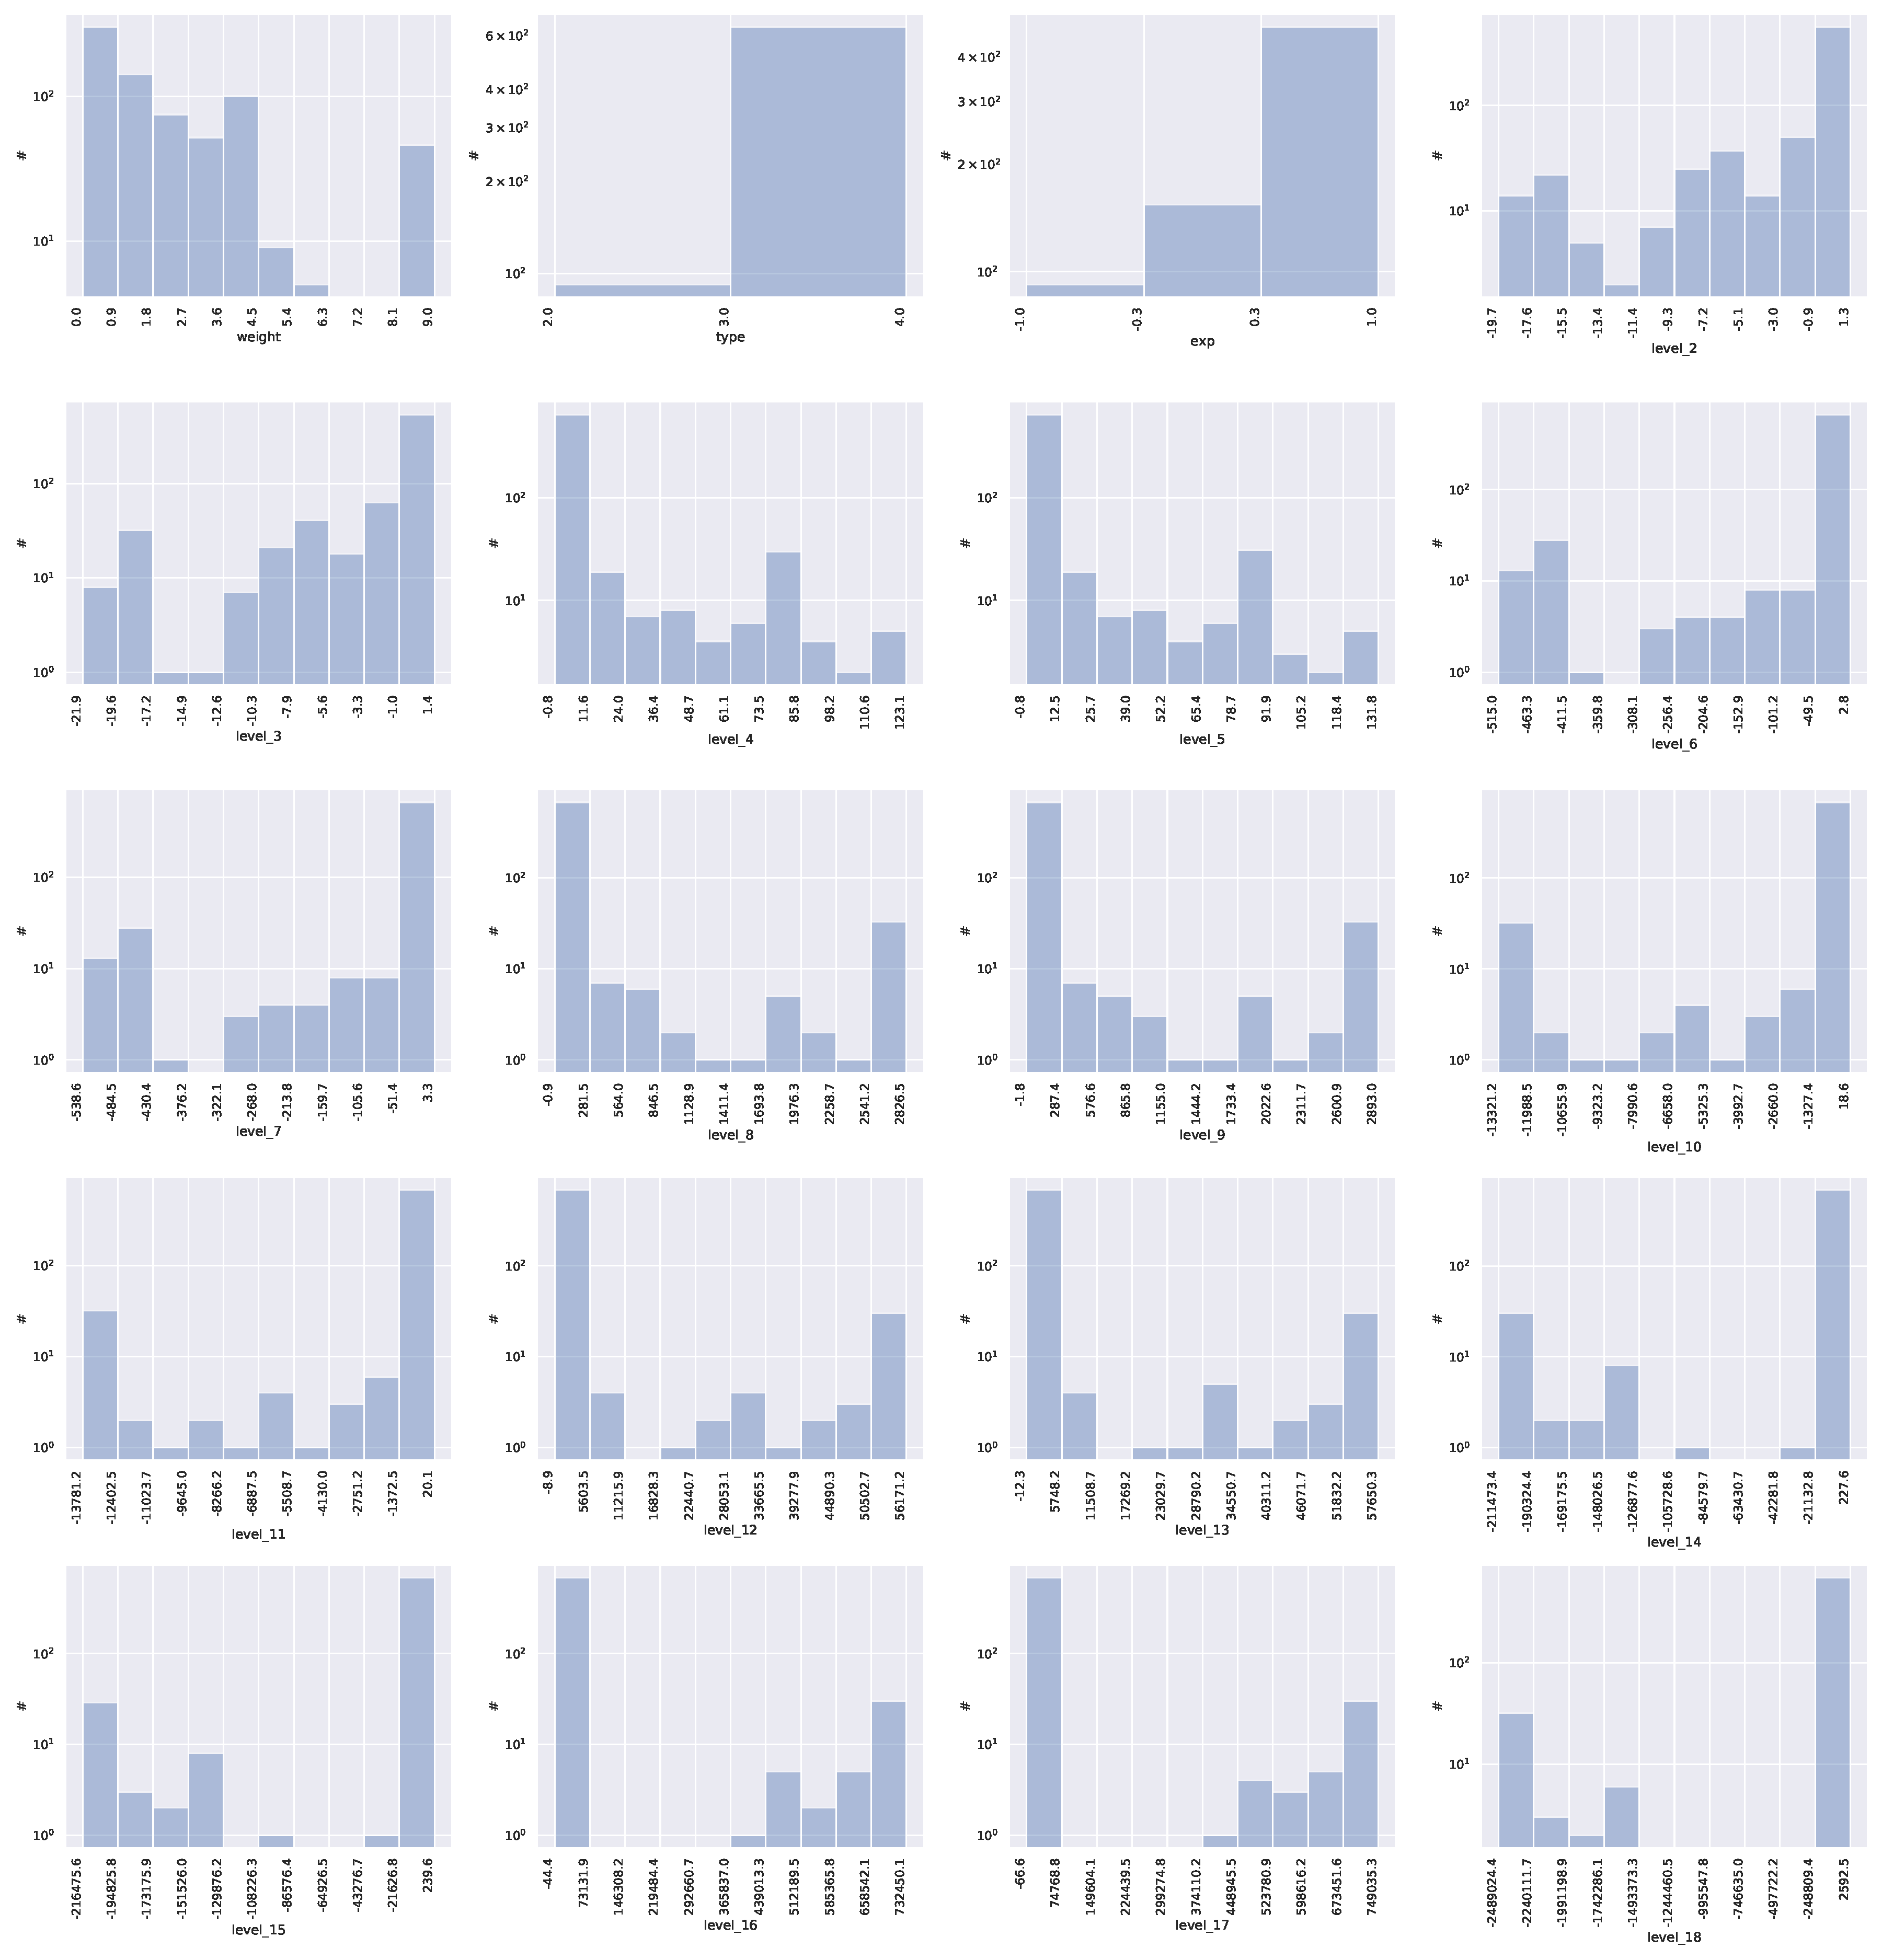
\includegraphics[width=0.4\textwidth]{img/dataset-distribution_full}
  \caption{Distribution of the variables in the dataset.}
  \label{fig:eda:distr_full}
\end{figure}
The distribution of the samples is summarised in \Cref{fig:eda:distr_full}: we
digitised each variable in at most 10 bins representing left-closed intervals
(i.e. $[a, b)$) between the values reported on the x-axis.
As we can see the distributions present a lot of outlying samples which may
lead to a ``artificially too small'' variance on the determination of the
coefficients of the regression.
The outliers are however mainly present in the distribution of the variables for which \texttt{weight} $\ge 1.5$.
\begin{figure}[htbp]
  \centering
  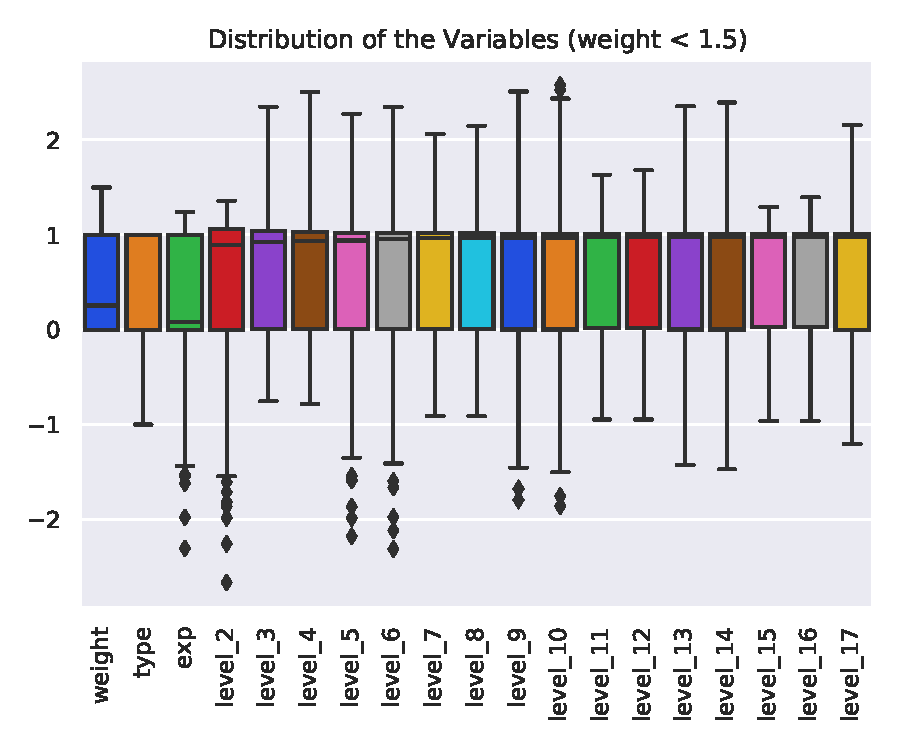
\includegraphics[width=0.4\textwidth]{img/dataset-distribution_box_low}
  \caption{Distribution of the variables for \texttt{weight} $< 1.5$.}
  \label{fig:eda:low_weight}
\end{figure}
In fact if we consider \texttt{weight} $< 1.5$ the variables are more
reasonably distributed, and might be easier to train in a following regression
analysis, as we show in \Cref{fig:eda:low_weight}.

\subsection{Correlations}\label{sec:eda:corr}

Following the outliers detection analysis, we first notice that for different
ranges of the \texttt{weight} variable, only certain types of oscillations are
present.
\begin{table}[htbp]
\centering
\begin{tabular}{@{}cccc@{}}
\toprule
                 &               & \multicolumn{2}{c}{\textbf{weight}} \\
\textit{range}   & \textit{type} & \textit{mean}  & \textit{variance}  \\
\midrule
weight $\ge 1.5$ & 4             & 4.03           & 5.13               \\
\midrule
\multirow{2}{*}
{weight $< 1.5$} & 2             & 0              & 0                  \\
                 & 4             & 0.58           & 0.21               \\
\bottomrule
\end{tabular}%
\caption{Type of oscillations per weight range.}
\label{tab:eda:weight}
\end{table}
In fact, in \Cref{tab:eda:weight} we show that for higher weights there is only
one type of oscillations in the dataset, while for lower weights the type 2
oscillation implies \texttt{weight} $= 0$ identically.

This in turns may also be reflected in the correlation between the variables.
This is defined for each possible couple of variables as the ration between
their covariance and the product of their separate standard deviations.
In \Cref{fig:eda:corr} we show the different correlation factors in a graphical
representation.
\begin{figure}[htbp]
  \centering
  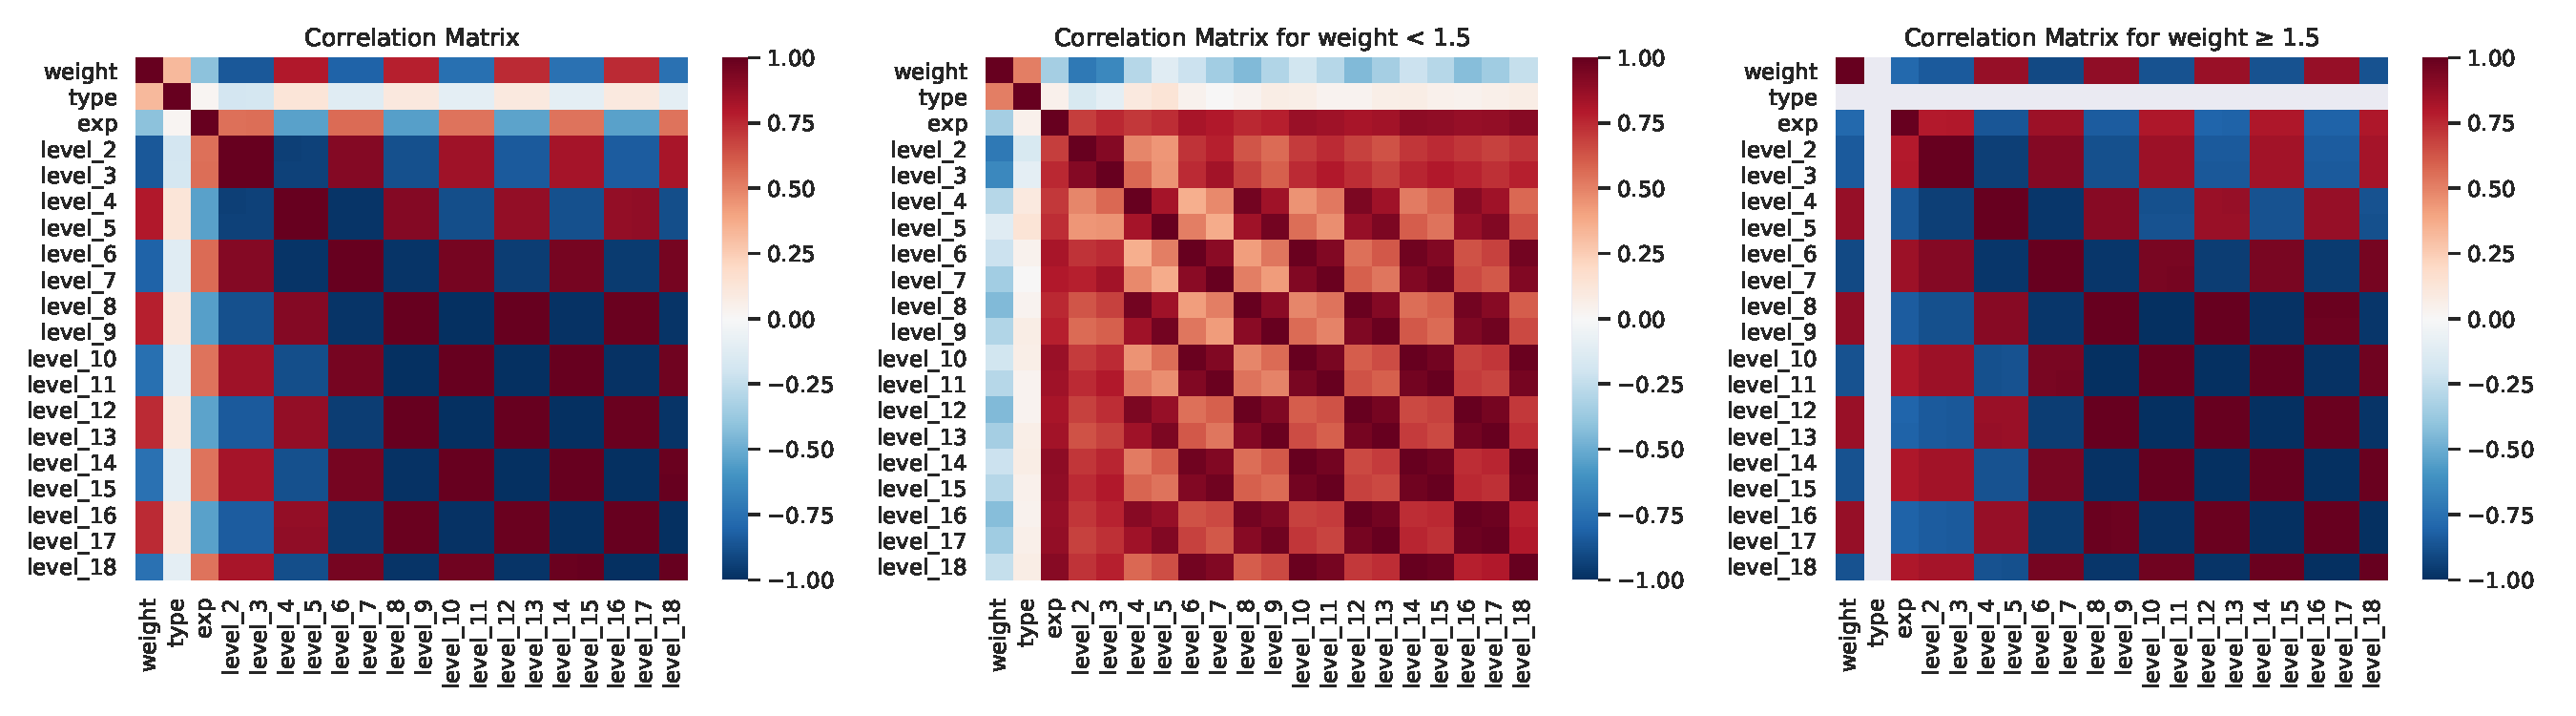
\includegraphics[width=0.4\textwidth]{img/corr-mat}
  \caption{Correlation matrix of the variables.}
  \label{fig:eda:corr}
\end{figure}
As expected, the truncation levels are strongly correlated among themselves and
with the \texttt{weight} variable.
Though milder, there is also a good correlation of the variables with the
labels we intend to predict (\texttt{exp}), while the \texttt{type} variable
seems to be completely uncorrelated (this may however be due to the fact of
being categorical: a linear regression might be more suitable to do statistical
inference on it).

\subsection{Principal Components Analysis}\label{sec:eda:pca}

We perform the Principal Components Analysis (PCA) of the truncation levels to
study their properties and their distribution.
We first study all its components using the Singular Value Decomposition (SVD)
of the matrix holding samples over the rows and the truncation levels over the
columns (it is a rectangular matrix and as such cannot be strictly diagonalised
to perform spectral analysis).
In \Cref{fig:eda:pca} we show the variance explained by each principal
component of the matrix (i.e.\ the fraction of variance of the total set
retained by considering only the selected component).
\begin{figure}[htbp]
  \centering
  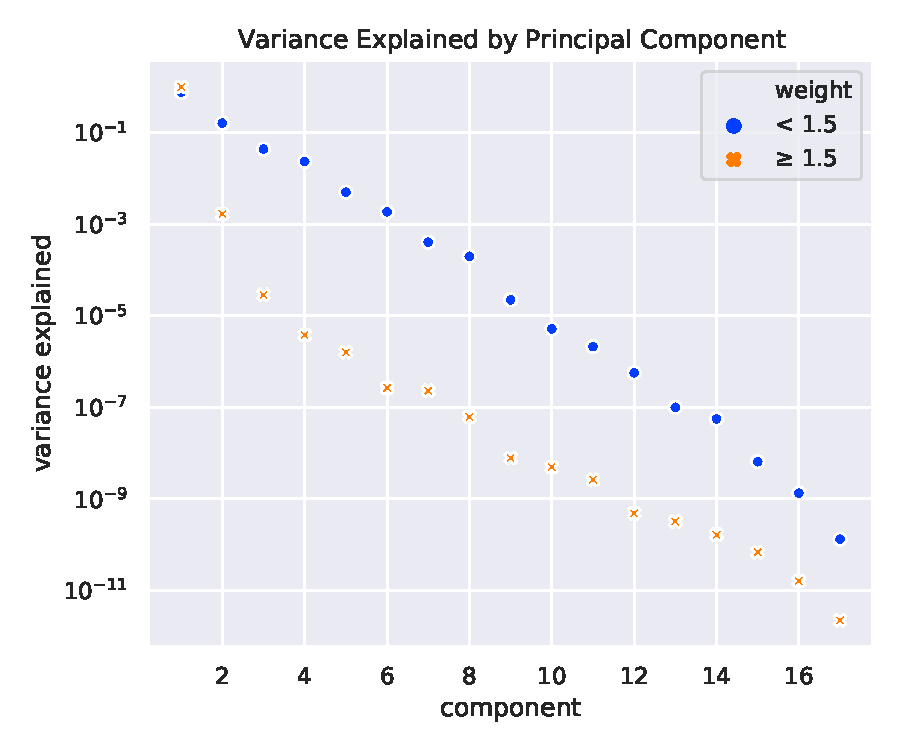
\includegraphics[width=0.4\textwidth]{img/pca-variance-explained}
  \caption{Variance explained by the principal components of the truncation levels (log scale).}
  \label{fig:eda:pca}
\end{figure}

The analysis was performed splitting the dataset over ranges of the
\texttt{weight} variable and shows that for lower weights the first two
principal components account for more than 90\% of the total variance of the
values, while for larger weights almost 100\% of the variance is explained by
the first component.
This reflects the distribution of the variables in the dataset: larger weights
contain a very large amount of outliers and have larger variance with respect
to lower weights, thus it might be enough to project the values of the
truncation levels over the line which contains most of the deviation to
reproduce a meaningful distribution.

\subsection{K-Means Clustering}\label{sec:eda:kmeans}

Finally we perform an unsupervised clustering analysis.
The main idea is to infer a structure in the data which may be able to
``automatically'' reproduce the labels (i.e.\ the \texttt{exp} column) without
regression.
In other words we study the distribution of the truncation levels and fit it in
3 clusters representing the 3 integer values of the labels.
In the ideal scenario there should be a 1:1 relation between the labels of the
cluster centroids and the labels in the \texttt{exp} variable. Unfortunately
the cluster analysis of the truncation levels over the entire dataset
highlighted no particular structure in the data and turned out inconclusive.

We then performed the same analysis splitting the dataset in different ranges
of the \texttt{weight} variable, standardising the data for \texttt{weight} $<
1.5$ and robustly scaling (i.e.\ scaling according the interquartile range)
samples for which \texttt{weight} $\ge 1.5$.
Based on the results of \Cref{sec:eda:pca}, in \Cref{fig:eda:kmeans} we used
the principal components of the truncation levels to plot the distribution of the clusters and the \texttt{exp} labels.
\begin{figure}[htbp]
  \centering
  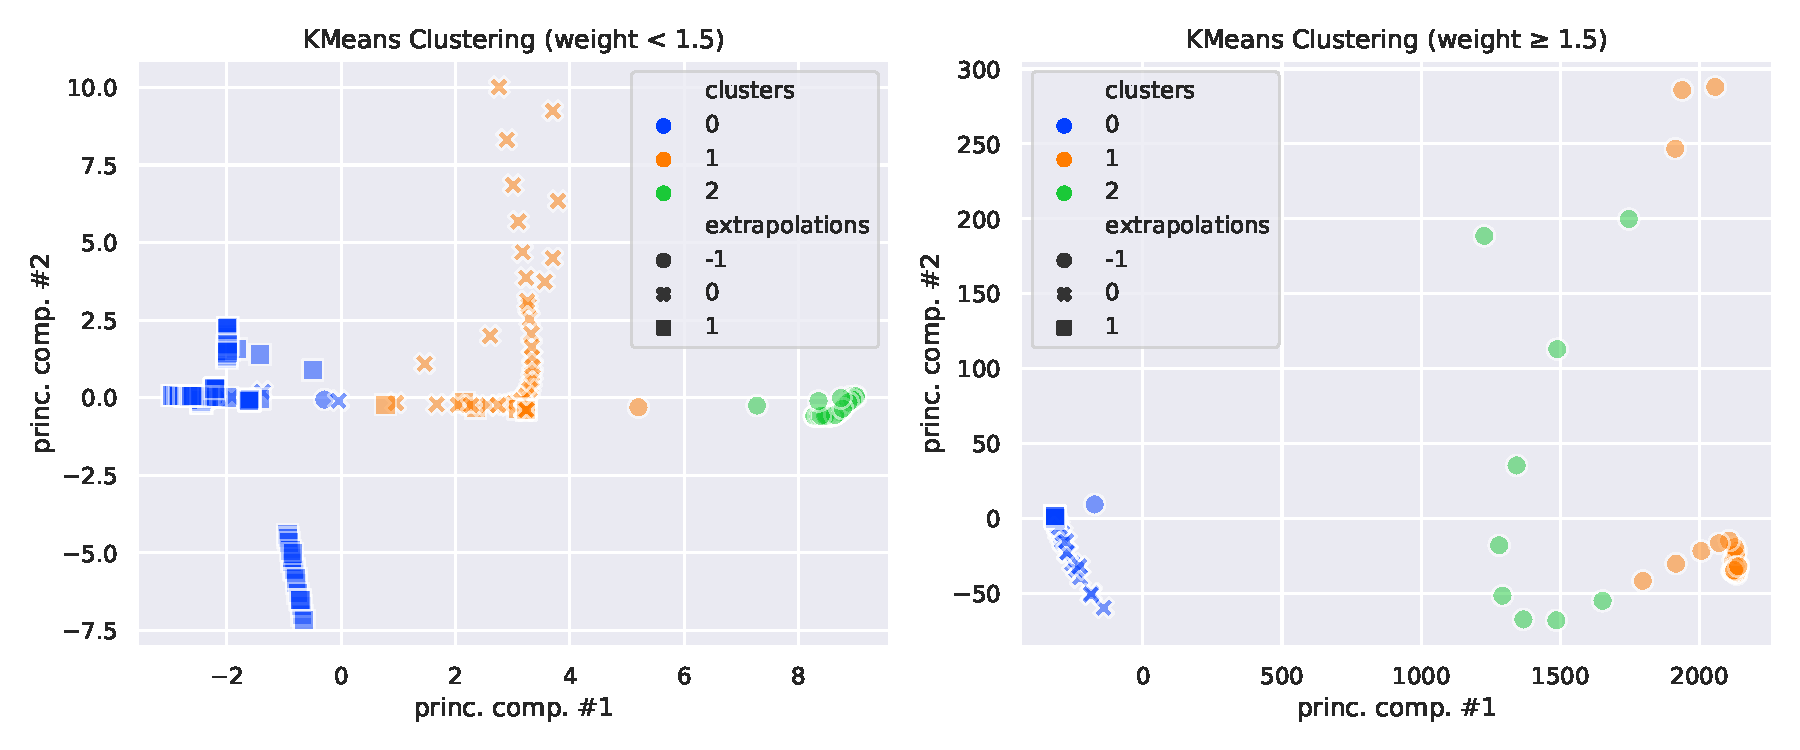
\includegraphics[width=0.475\textwidth]{img/kmeans-clusters}
  \caption{K-Means clusters and \texttt{exp} labels plotted using the principal
  components for visualisation purposes.}
  \label{fig:eda:kmeans}
\end{figure}
As we can see, recognising a structure is challenging when \texttt{weight} $\ge
1.5$ and in fact different \texttt{exp} (or ``extrapolation'') labels generally
belong to different clusters.
However the case \texttt{weight} $< 1.5$ seems to be more accurate and shows
that in general we can recognise a structure in the data.
\begin{table}[htbp]
\centering
\begin{tabular}{@{}cccc@{}}
\toprule
                     &              & \multicolumn{2}{c}{\textbf{weight}}   \\
\midrule
\textit{clusters}    & \textit{exp} & \textit{$< 1.5$} & \textit{$\ge 1.5$} \\
\midrule
\multirow{3}{*}
{average label} & -1 & 1.84             & 1.13               \\
                     & 0            & 0.92             & 0.00               \\
                     & 1            & 0.02             & 0.00               \\
\bottomrule
\end{tabular}%
\caption{Average cluster label per weight range.}
\label{tab:eda:kmeans}
\end{table}
In \Cref{tab:eda:kmeans} we recognise that there is a distinguishable relation
between the extrapolation column and the average cluster label in the group
when \texttt{weight} $< 1.5$, while in general there is a superposition of
labels when \texttt{weight} $\ge 1.5$ (it seems that there are only 2
recognisable clusters).


  \section{Regression Analysis}\label{sec:reg}
    In what follows we decided to drop the first type of solution from the dataset
(i.e.\ \texttt{solutions} $= 0$) since it looks ``too perfect'' for the
analysis and might spoil the final results (also, removing a restricted number
of samples does not change the underlying distribution, as shown earlier).

\subsection{Test and Validation Sets}\label{sec:reg:test_val}

The splits for training and test sets have been chosen in order to keep samples
coming from the same \texttt{solutions} inside the same set in order to
maintain a good balance in the distribution of the variables.
In other words, we choose the samples in the test and training sets by first
subsampling the unique values of the \texttt{solutions} column, then we split
them into separate sets, and ultimately we assign the corresponding samples to
the splits.
The size of the splits has been chosen to optimise the trade-off between the
number of samples (which is very restricted and requires the largest split to
be assigned for training) and the possible error (identified by the Mean
Squared Error, or MSE from now on).

\begin{figure}[htbp]
  \centering
  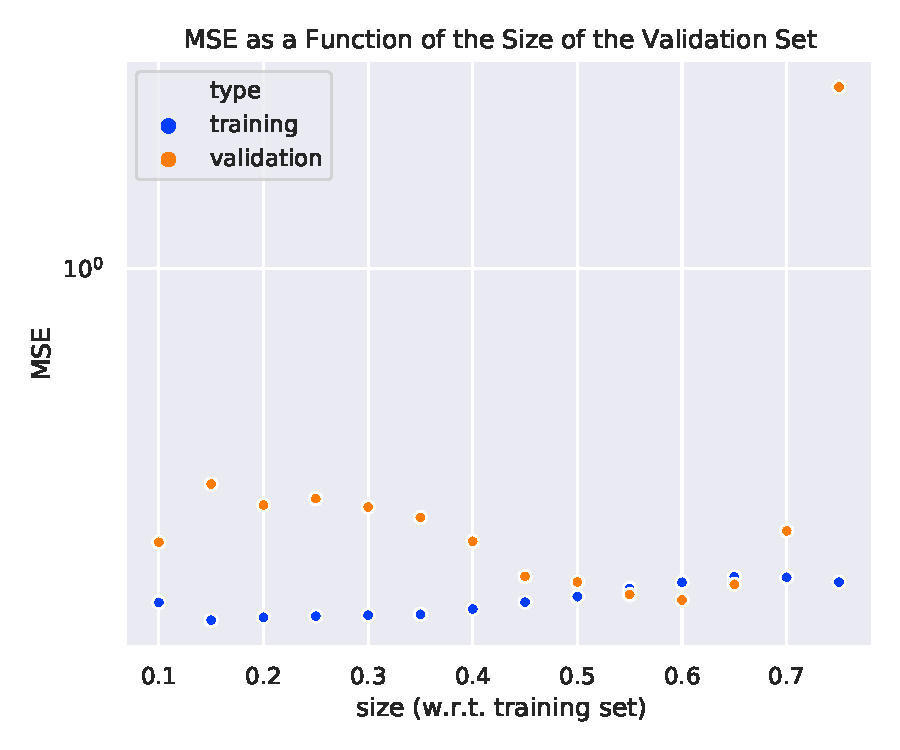
\includegraphics[width=0.4\textwidth]{img/training-validation-errors}
  \caption{MSE in training and validation for several sizes of the validation set.}
  \label{fig:reg:validation_size}
\end{figure}
We first decide to subsample around 10\% of the solutions for the test set and
keep the remaining 90\% for training and validation.
Notice that we do not use cross-validation in this case since the number of
samples is very restricted and we still want to keep samples coming from the
same \texttt{solutions} in the same split.

The size of the validation set has been chosen to minimise the error made when
fitting a linear regression on decreasing size of the set effectively used for
training, after removing the validation split.
In \Cref{fig:reg:validation_size} we show training and validation MSE for
different sizes of the validation set (with respect to the total training set).
In order to keep a reasonable amount of samples in the training split and to
contain the validation MSE as much as possible, we take the 10\% of the unique
\texttt{solutions} in the validation set.
\begin{table}[htbp]
\centering
\begin{tabular}{@{}ccc@{}}
\toprule
           & \multicolumn{2}{c}{\textbf{total dataset}} \\
\midrule
           & \textit{samples}    & \textit{fraction}    \\
\midrule
training   & 579                 & 81\%                 \\
validation & 61                  & 8\%                  \\
test       & 78                  & 11\%                 \\
\bottomrule
\end{tabular}
\caption{Summary of the train/validation/test splits.}
\label{tab:reg:splits}
\end{table}
In \Cref{tab:reg:splits} we give a schematic summary of the final choice for
training, validation and test sets.

\subsection{Preliminary Linear Regression Analysis}\label{sec:reg:prel}

Before moving to the ML analysis, we first perform a preliminary study using
linear regression to infer properties of the variables which may play a role in
the ML algorithms.
From now on we shall consider the training data as robustly scaled against the
outliers (i.e.\ we pre-process using \texttt{sklearn.RobustScaler}). 

We first fit the linear regression algorithm on the train set and then compute
the predictions on the three splits to study the values of the coefficients
(full details can be found in the notebook in the
\href{https://github.com/thesfinox/ml-sft-trunc}{GitHub repository}), their
associated standard error, t-statistics and probabilities of being different
from zero.
For this and the ML analysis we do not fit the intercept of the models since
the variables cannot vanish altogether: the intercept has therefore no
interpretation in discovering a structure in the values or performing
regression.

The study revealed that when considering the full dataset, all the variables
should be considered for regression as the coefficients are non vanishing (with
95\% confidence), mostly due to the very large variance of the data which
allows only very precise (i.e.\ very small standard errors) determinations of
the coefficients.
The same study performed on the usual separate ranges of \texttt{weight} showed
that when considering \texttt{weight} $\ge 1.5$ the variable \texttt{type} is
not necessary to the fit and we cannot reject the hypothesis of a vanishing
coefficient for such feature: this in fact reflect one of the properties
discovered during the EDA and summarised in \Cref{tab:eda:weight} where we
showed that for \texttt{weight} $\ge 1.5$ only one \texttt{type} is present in
the dataset and does not influence the final predictions.
We will however keep such feature inside the training variables since a further
study on the full dataset without the categorical variable showed that
predictions are in general worse than in the previous cases (i.e.\ the
\texttt{type} variable helps when \texttt{weight} $< 1.5$).


  \section{Machine Learning Analysis}\label{sec:ml}
    In this section we briefly summarise the results of the ML analysis performed
on the data.
We will explore several diverse algorithms including regularised versions of
the linear regression (LR, from now on), support vector machines (SVM),
decision trees (random forests, RF, and gradient boosted decision trees, GBDT),
and artificial neural networks (ANN).
For each algorithm we fit the data on training set and evaluate it on the
validation set to perform the optimisation of the \textit{hyperparameters}
using Bayes statistics.
The goal is to minimise the objective function, that is the validation MSE,
without knowing its analytic form, by only inferring the probability of
obtaining a better result with a different choice of hyperparameters.

\subsection{Regression Analysis}\label{sec:ml:regr}

In \Cref{tab:ml:test} we summarise the results obtained from prediction on the
test set for the algorithms used: in particular the first four lines refer to
linear models (LR is the plain regression, EN implements both $l_1$ and $l_2$
regularisation, Lasso and Ridge separately implement $l_1$ and $l_2$
regularisation, respectively); l-SVR is the linear implementation of the SVM
models, while r-SVR uses a Gaussian \textit{kernel trick}; RF and GBDT are
different ensemble algorithms based on decision trees (namely random forests
and gradient boosted trees); ANN represents the neural network architecture (no
hidden layers, only one input layer with 30 units, batch normalisation layer
and a dropout layer with 0.1 drop rate leading to a network of 691 trainable parameters and 60 fixed parameters).

\begin{table}[htbp]
\centering
\resizebox{0.475\textwidth}{!}{%
\begin{tabular}{@{}lcccc@{}}
\toprule
         &             MSE &              MSE 95\% CI &  MAE &                   R2 \\
\midrule
LR       &            0.13 &           $[0.07, 0.20]$ & 0.27 &                 0.74 \\
EN       &            0.19 &           $[0.12, 0.27]$ & 0.33 &                 0.62 \\
Lasso    &            0.20 &           $[0.13, 0.28]$ & 0.34 &                 0.60 \\
Ridge    &            0.13 &           $[0.07, 0.20]$ & 0.27 &                 0.74 \\
l-SVR    & $8 \times 10^3$ & $[-3, 20] \times 10^{3}$ &   20 & $-1.6 \times 10^{4}$ \\
r-SVR    &           0.030 &                      --- & 0.08 &                 0.95 \\
RF       &           0.013 &                      --- & 0.05 &                 0.97 \\
GBDT     &          0.0010 &                      --- & 0.02 &                 1.00 \\
ANN      &           0.006 &                      --- & 0.05 &                 0.99 \\
\bottomrule
\end{tabular}
}
\caption{Summary of the predictions on the test set for the different
algorithms. We present the MSE, the Mean Absolute Error (MAE) and the
$R^2$ score. The confidence intervals of the MSE are present only for linear
models since they rely on statistical assumptions on the distribution of the
residuals (they are normally distributed).}
\label{tab:ml:test}
\end{table}

\begin{figure}[htbp]
  \centering
  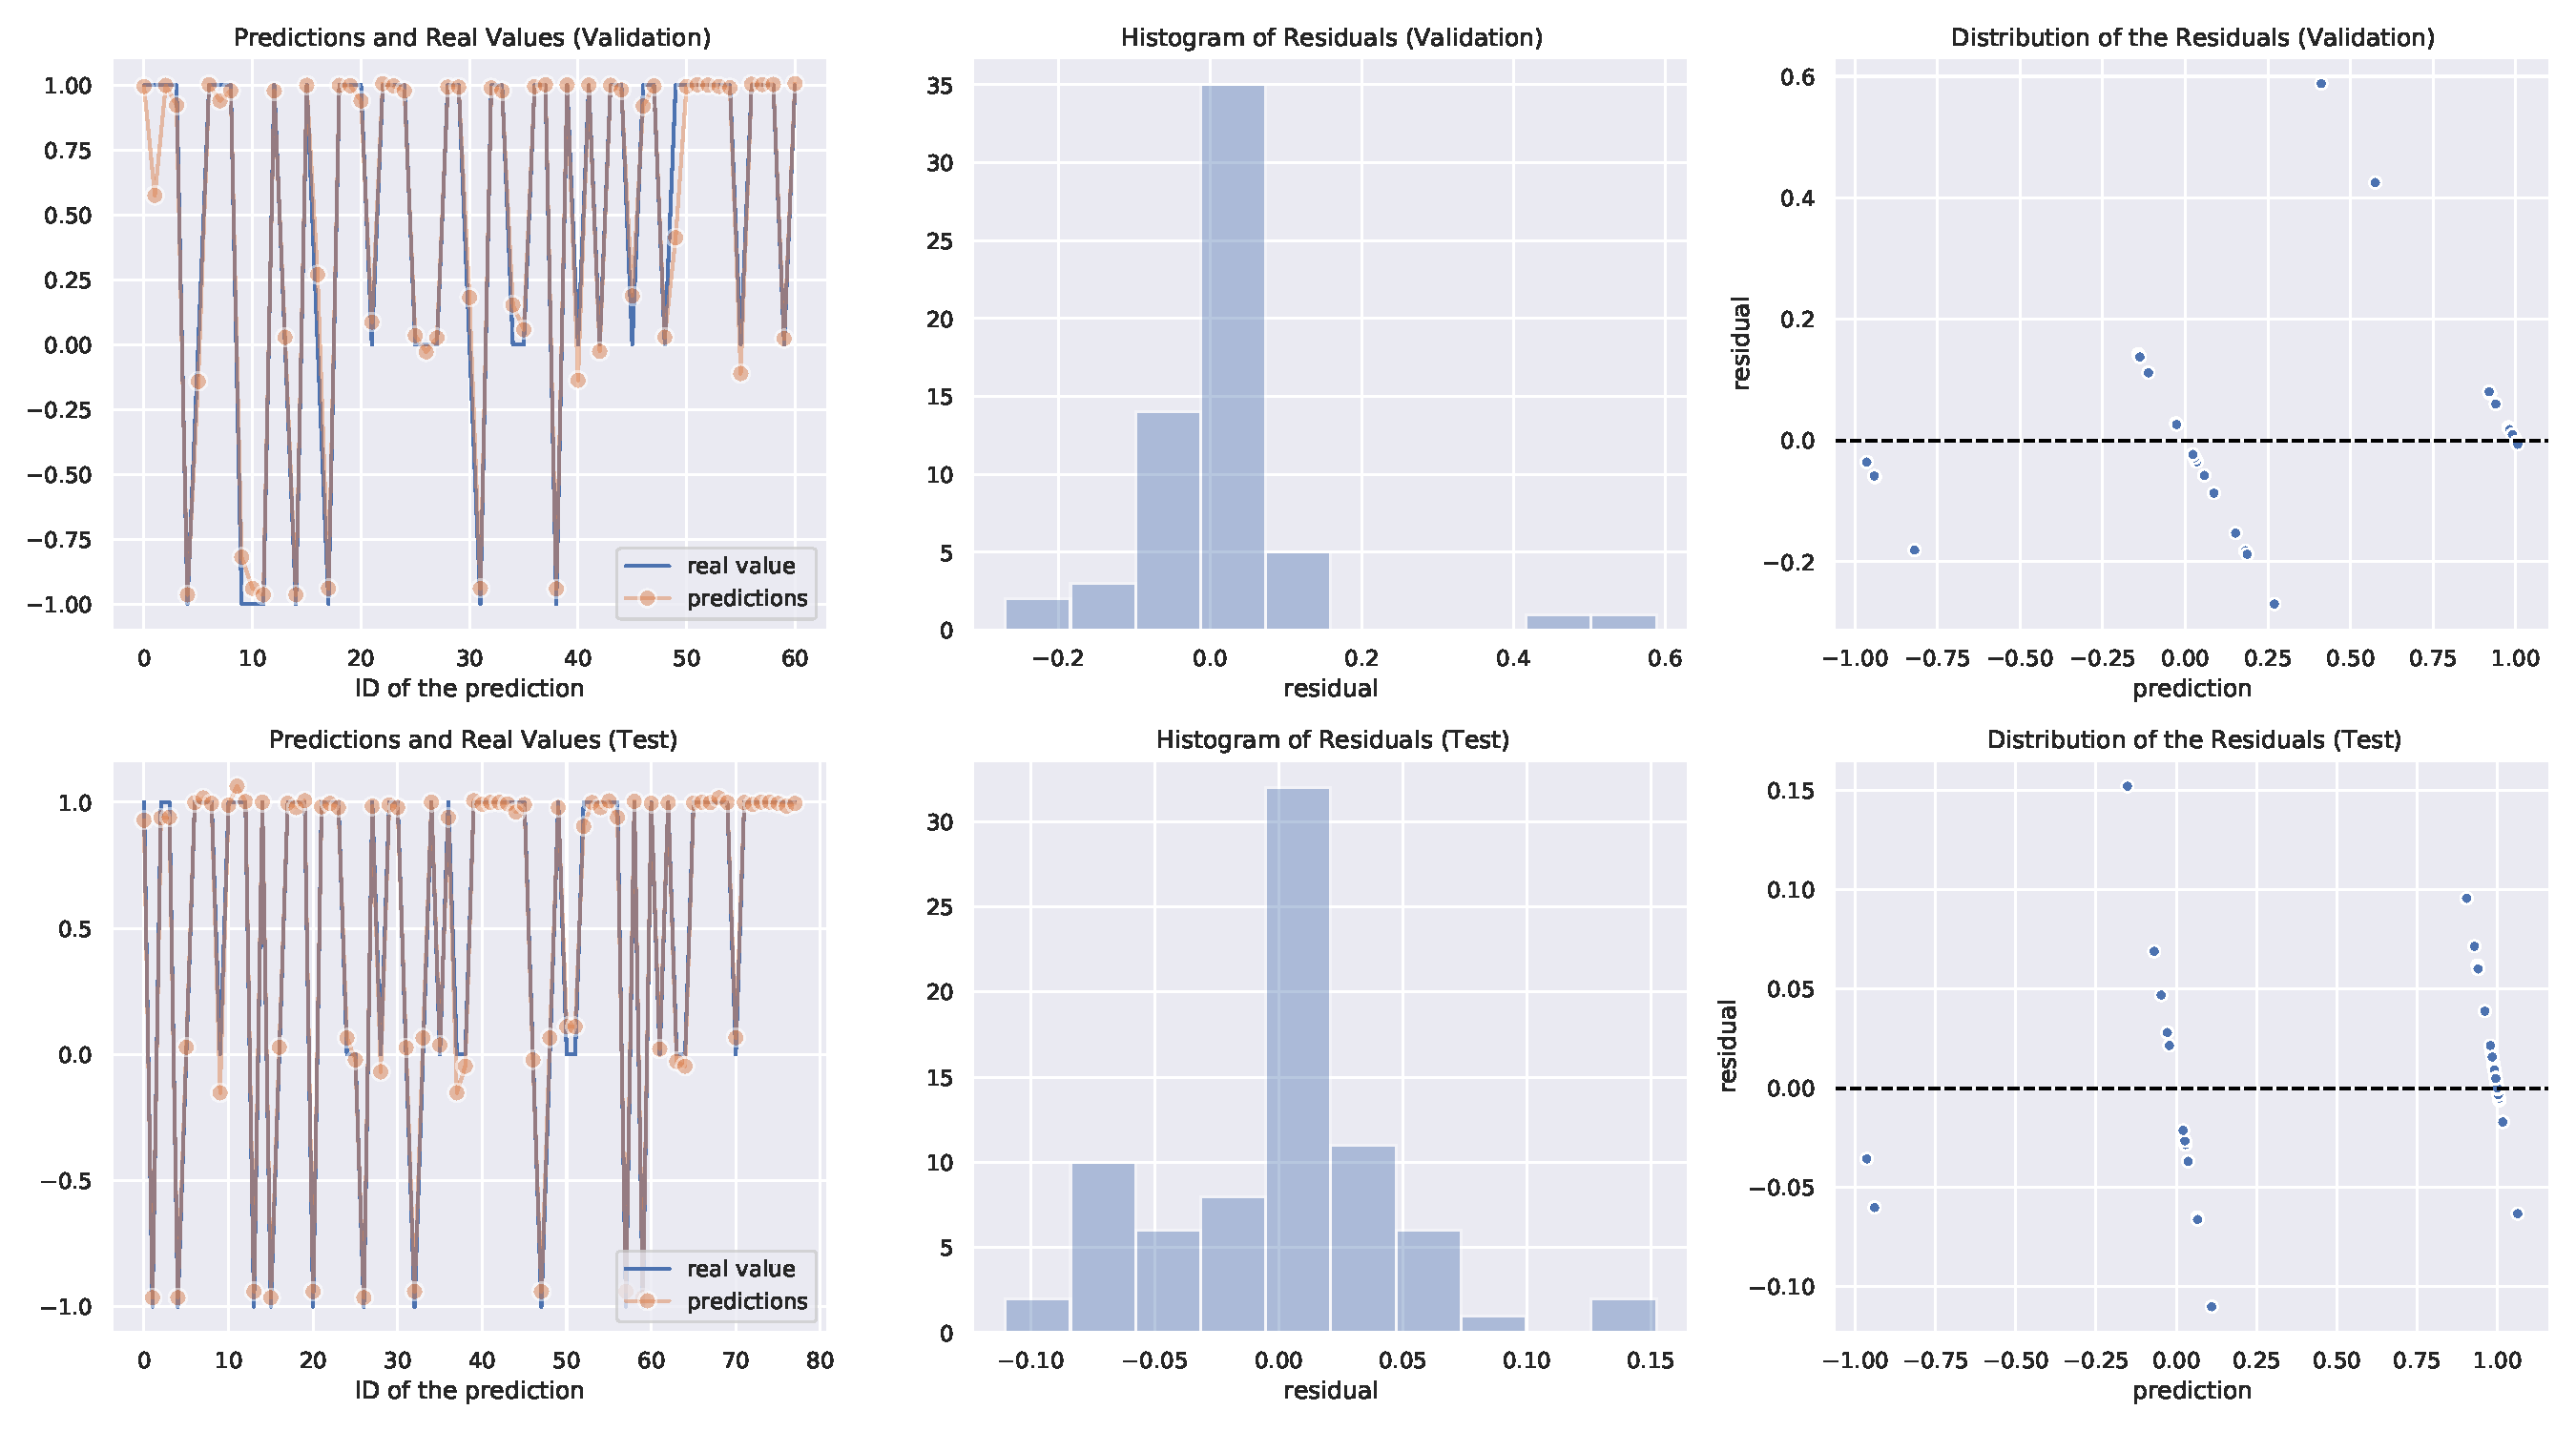
\includegraphics[width=0.475\textwidth]{img/grd_bst}
  \caption{GBDT validation and test sets residuals.}
  \label{fig:ml:gbdt}
\end{figure}

As we can see the GBDT are able to deliver the best results both in
terms of MSE and R2 score followed by the implementation of the shallow
network (trained over 5000 epochs: training is fairly rapid but trees are by
far faster).
On the other hand $l_1$ regularisation (both alone and in combination with
$l_2$) fails to approximate well the prediction labels. In the same fashion the
l-SVR fails completely.

In \Cref{fig:ml:gbdt} we show the validation and test set distribution of the
predictions and residuals.
As we can see the algorithm correctly approximates the \texttt{exp} labels with
residual contained in a small interval.
There is however a general tendency to underestimate the \texttt{exp} $= -1$
label and to overestimate \texttt{exp} $= 1$: in linear model this would have
signalled an incomplete model since residuals seem to be correlated with
predictions, but in the case of decision trees it does not pose an issue.

\begin{figure}[htbp]
  \centering
  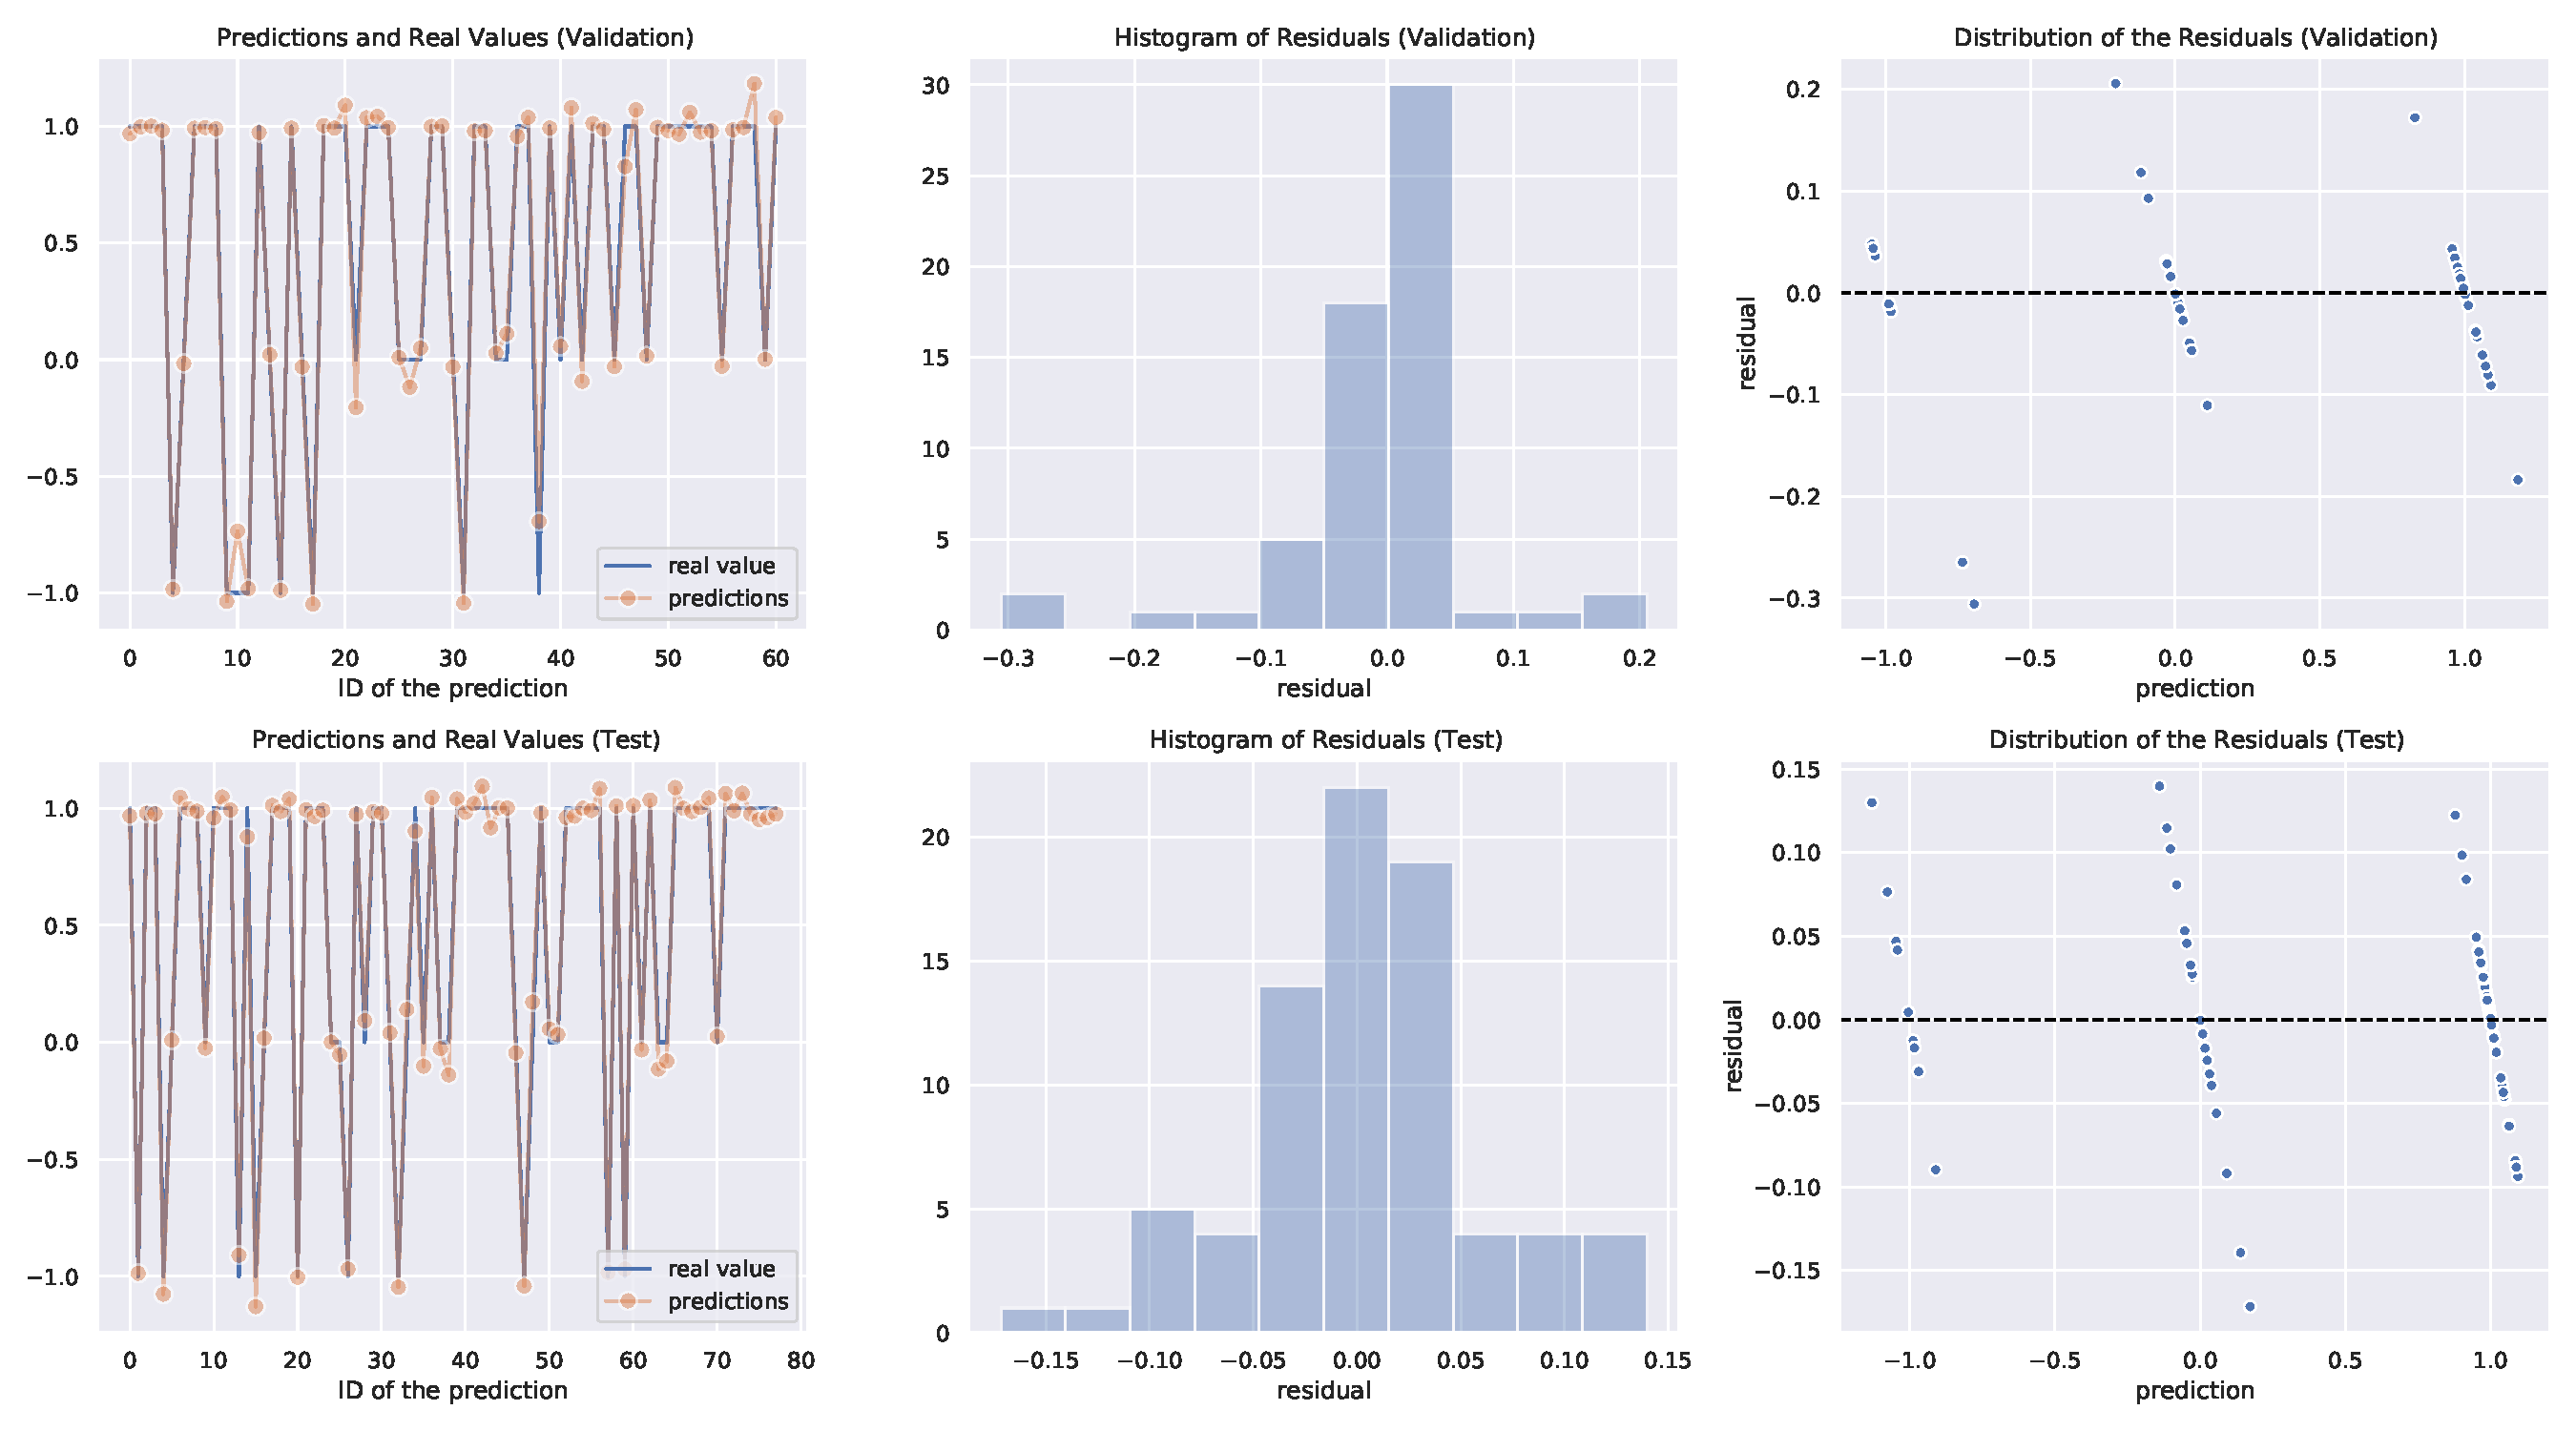
\includegraphics[width=0.475\textwidth]{img/ann_mod}
  \caption{ANN validation and test sets residuals.}
  \label{fig:ml:ann}
\end{figure}

In \Cref{fig:ml:ann} we show the same plot generated from the ANN predictions.
As for the GBDT, the ANN is correctly trying to predict the \texttt{label} with
very small residuals.
Differently from the GBDT, residuals are more randomly distributed for each
prediction and no pattern is recognisable.

\begin{table}[htbp]
\centering
\begin{tabular}{@{}lcc@{}}
\toprule
                  & \textbf{RF} & \textbf{GBDT} \\
\midrule
no.\ leaves       & 48          & 15            \\
max depth         & 300         & 17            \\
no.\ estimators   & 25          & 3439          \\
subsample         & 0.85        & 0.99          \\
colsample by tree & 0.7         & 1.0           \\
min child weight  & 0.01        & 0.1           \\
$l_1$ reg.        & 0.16        & 1.0           \\
$l_2$ reg.        & 0.20        & $10^3$        \\
learning rate     & ---         & 0.1           \\
\bottomrule
\end{tabular}%
\caption{Hyperparameters choices for RF and GBDT.}
\label{tab:ml:hyper}
\end{table}

In \Cref{tab:ml:hyper} we show a summary of the hyperparameters used for
training RF and GBDT: as expected the optimisation process chose a small number
of fully grown trees in the first case, while it led to a large number of
boosting rounds of shallow trees in the latter.

\subsection{Feature Explanation}\label{sec:ml:shap}

As a last step in the analysis, we use the trained trees (for simplicity) and
study their properties to possibly show how each training feature plays inside
the algorithm and how the final prediction is determined.
For this analysis we will study the Shapley values computed as the difference
between each permutation of subsamples of the features and compare the results
with the average of the final prediction in order to see which variable is
pushing the results and which variable is dragging it.
We will also consider the variable ranking provided naturally by the decision trees to determine which feature plays a larger role for the final prediction.

\begin{figure}[htbp]
  \centering
  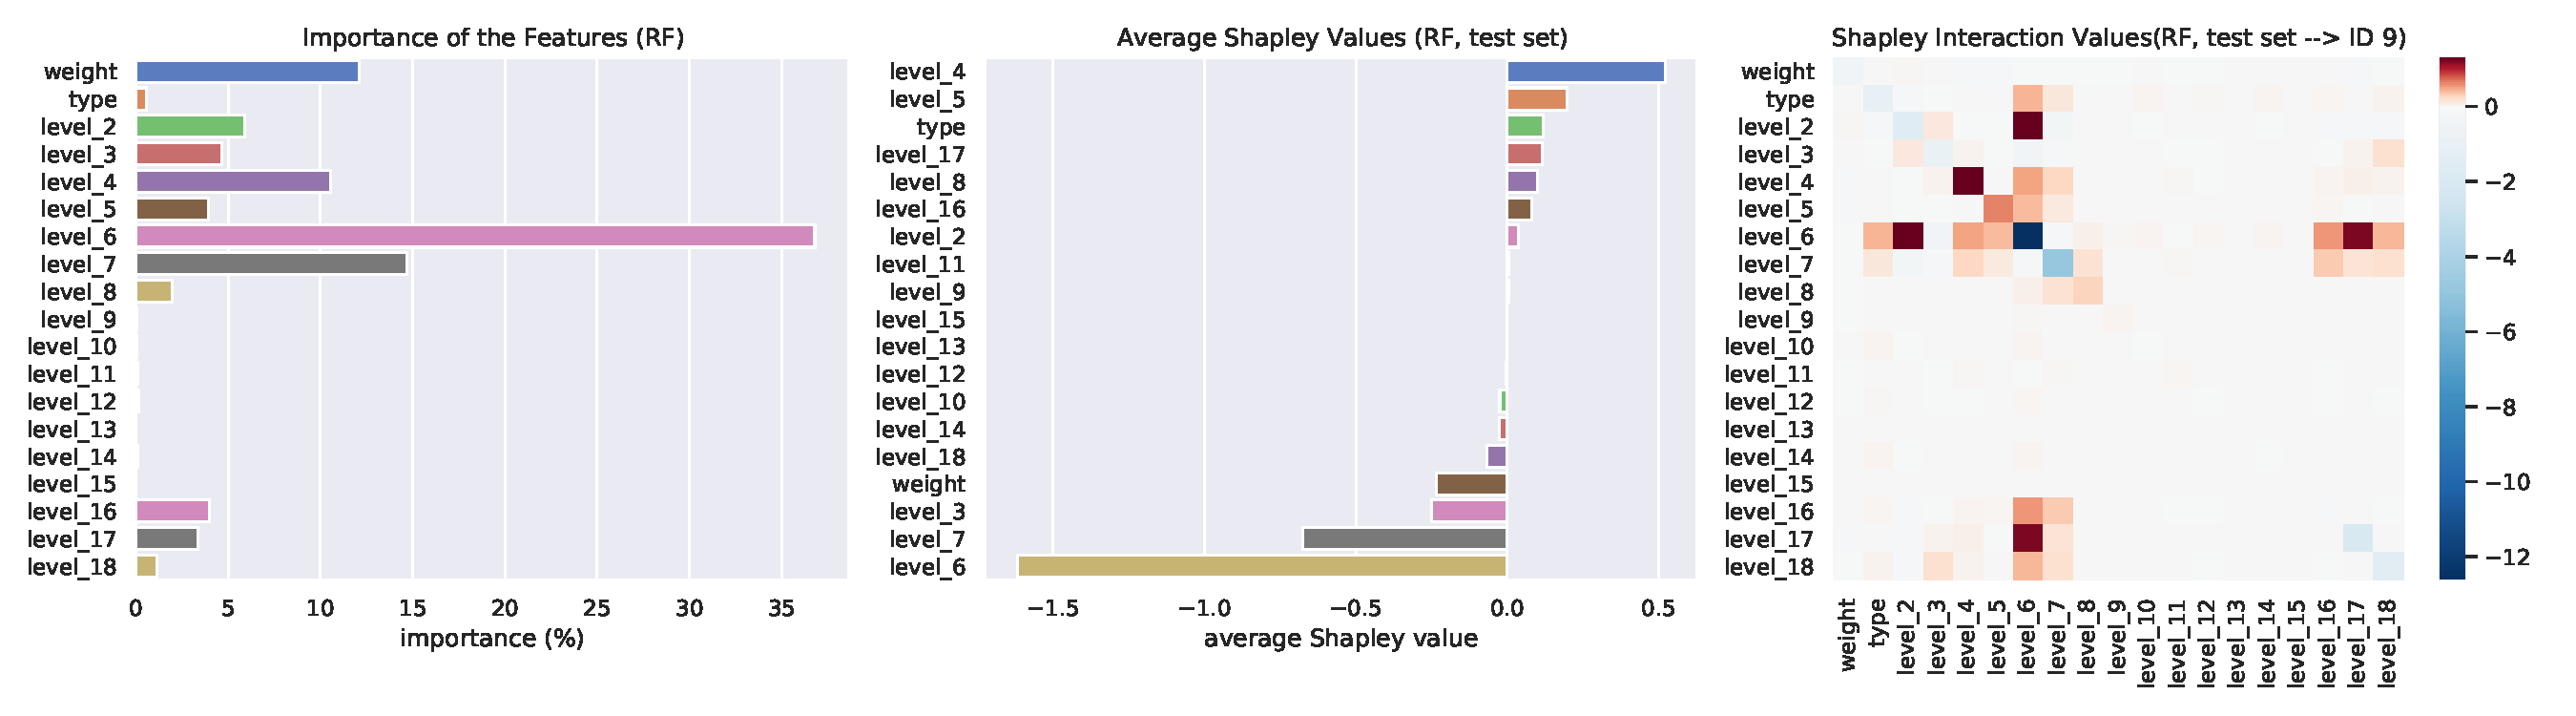
\includegraphics[width=0.475\textwidth]{img/rnd_for_shapley}
  \caption{Variable ranking and Shapley values (computed on the test set) of
  RF.}
  \label{fig:ml:rnd_for_shap}
\end{figure}

In \Cref{fig:ml:rnd_for_shap} we show the variable ranking and the Shapley
values for the RF algorithm.
The first plot shows that RF rely mostly on low and high truncation orders in
the top levels of the trees to better discriminate the predictions, even though
\texttt{weight} is still the most important feature (as we could have expected
from the results of the EDA).
The average Shapley values (second plot) show that most features give a comparable contribution to the prediction, exception made for one of them which seems to drive the final result in a more direct way.
Finally the \textit{interacting Shapley values} (taken for a random sample in
the test set) in the third plot show that the whole set of variables is mostly
non interacting except very sporadic contributions between distant levels.

\begin{figure}[htbp]
  \centering
  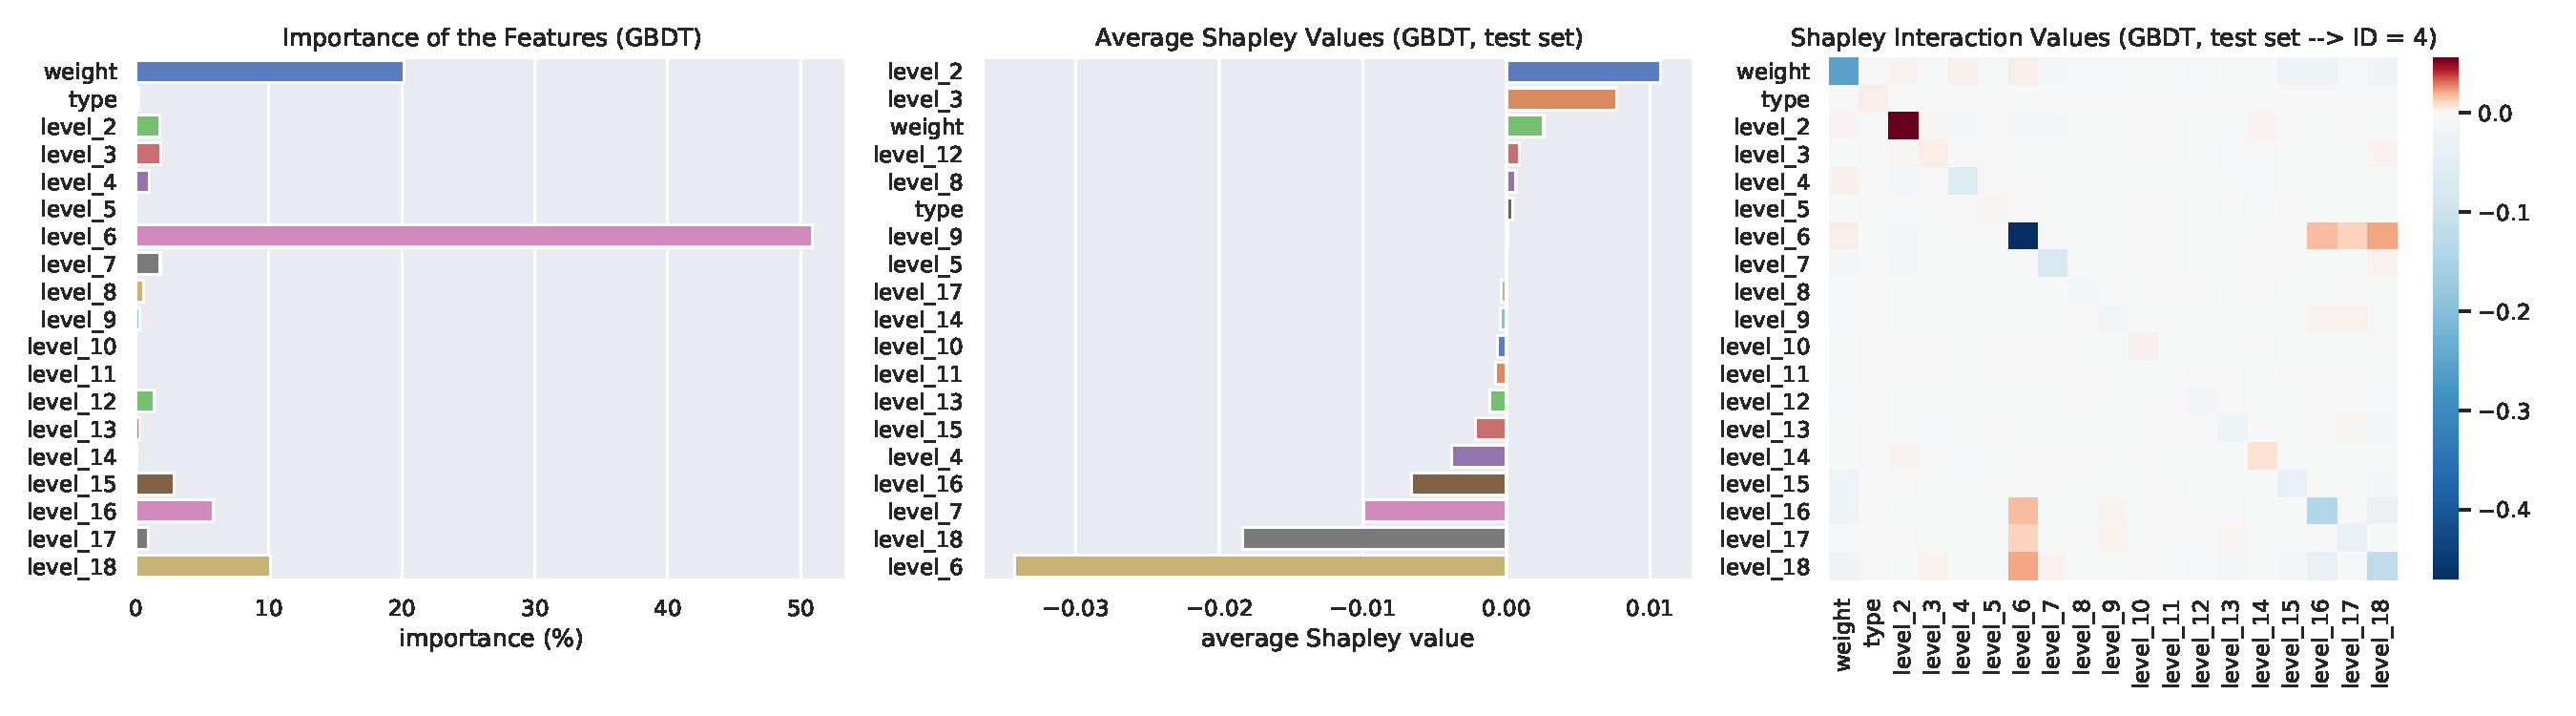
\includegraphics[width=0.475\textwidth]{img/grd_bst_shapley}
  \caption{Variable ranking and Shapley values (computed on the test set) of GBDT.}
  \label{fig:ml:grd_bst_shap}
\end{figure}

In \Cref{fig:ml:grd_bst_shap} we finally show the same plot for the GBDT.
Differently from the RF, GBDT seem to attach greater importance also to the
central truncation levels while disregarding almost completely the categorical
variable (for this particular algorithm it could have been removed but the
corresponding Shapley value shows that its relevance is so marginal that the
result would not have changed).


  \section{Conclusions}\label{sec:concl}
    We showed that the dataset has an heterogeneous and sparse distribution when
not accounting for the range of the \texttt{weight} variable.
In particular, in the case of low weight the distribution is contained and
shows an underlying distribution which unsupervised learning can capture and
connect to the prediction labels.
Discriminating over the \texttt{weight} variable also revealed that some
choices of the \texttt{type} variable are somewhat forced (see
\Cref{tab:eda:weight}), leading to consequences in the analysis of linear
regression in \Cref{sec:reg:prel}.
The ML analysis revealed that the best algorithms for the prediction of the
labels are GBDT and ANN which reproduce correctly and without overfitting (we
did not show explicitly the numbers, but the validation MSE are comparable to
the test results shown in \Cref{tab:ml:test}).
We finally showed how decision trees treat each variable during predictions on
the test set and revealed that features rarely influence each other.
In general the predictions of the trees and the ANN seem to be reliable and
consistent, suggesting that indeed the prediction of the \texttt{exp} labels is
an achievable task.


  \printbibliography

\end{document}
